\chapter{Software and Hardware Implementation of a Watermarking Scheme using CIPRNG}
\label{Application Example}
\minitoc



%Cryptographically secure PRNGs are fundamental tools to communicate through the Internet. Original and encrypted image are shown in Fig.\ref{Distribution of original image}(a) and 
%Fig.\ref{Distribution of encrypted image}(a), whereas Fig.\ref{Distribution of original image}(b) and Fig.\ref{Distribution of encrypted image}(b) depict their histograms. 
%Obviously the distribution of the encrypted image is very close to the uniform distribution, which improves the protection against statistical attacks.
%
%
%
%
%
%\begin{figure*}
%\begin{minipage}[b]{.48\linewidth}
%\centering
%\centerline{\epsfig{figure=lena.eps,width=5cm}}
%\centerline{(a) Original image.}
%\end{minipage}
%\hfill
%\begin{minipage}[b]{0.48\linewidth}
%\centering
%\centerline{\epsfig{figure=Histogram_lena.eps,width=8cm}}
%\centerline{(b) Histogram.}
%\end{minipage}
%\caption{Distribution of original image}
%\label{Distribution of original image}
%\end{figure*}
%
%\begin{figure*}
%\begin{minipage}[b]{.48\linewidth}
%\centering
%\centerline{\epsfig{figure=lena_crypt.eps,width=5cm}}
%\centerline{(a) Encrypted image.}
%\end{minipage}
%\hfill
%\begin{minipage}[b]{0.48\linewidth}
%\centering
%\centerline{\epsfig{figure=Histogram_lena_crypt.eps,width=8cm}}
%\centerline{(b) Histogram.}
%\end{minipage}
%\caption{Distribution of encrypted image}
%\label{Distribution of encrypted image}
%\end{figure*}
%
%Fig.\ref{Correlation distributions of two horizontally adjacent pixels in the original image and the encrypted image} shows the correlation distribution of two horizontally adjacent pixels, both in the original and in the encrypted images. Correlation coefficients in the horizontal, vertical, and diagonal directions concerning these two images are presented in Tab.\ref{Correlation coefficients of two adjacent pixels in the original image and the encrypted image}. Obviously, the correlation is important in the original image, whereas it is low and can be ignored in the encrypted image. These simple illustrations tend to prove that the use of CI PRNGs for cryptographic applications can be studied, to determine whether these chaotic generators is cryptographically secure working at the application or not. These study has been partially initiated in \cite{guyeuxTaiwan10,bgw10:ip,bfgw11:ij,bfg12b:ip}, in which our generators have been used as a component of watermarking scheme. The robustness of this scheme 
%has been evaluated, which has led to results as good as possible, thus reinforcing our opinion that these generators would probably be useful in cryptographic applications.
%The question of whether CI PRNGs are working application well or not, will thus be raised in our next work.
%
%\begin{figure*}
%\begin{minipage}[b]{.48\linewidth}
%\centering
%\centerline{\epsfig{figure=Correlation_distribution_of_the_original_image.eps,width=8cm}}
%\centerline{(a) Original image.}
%\end{minipage}
%\hfill
%\begin{minipage}[b]{0.48\linewidth}
%\centering
%\centerline{\epsfig{figure=Correlation_distribution_of_the_encrypted_image.eps,width=8cm}}
%\centerline{(b) Encrypted image.}
%\end{minipage}
%\caption{Correlation distributions of two horizontally adjacent pixels}
%\label{Correlation distributions of two horizontally adjacent pixels in the original image and the encrypted image}
%\end{figure*}
%
%\begin{table*}
%\renewcommand{\arraystretch}{1.3}
%\caption{Correlation coefficients of two adjacent pixels in the original image and the encrypted image}
%\label{Correlation coefficients of two adjacent pixels in the original image and the encrypted image}
%\centering
%\begin{tabular}{ccc} \toprule
%\textbf{Direction} &\textbf{Original image} & \textbf{Encrypted image} \\ \midrule
%Horizontal &0.9245 &-0.0059 \\
%Vertical &0.9617 &-0.0048 \\
%Diagonal &0.8967 &-0.0052 \\ \bottomrule
%\end{tabular}
%\end{table*}


\section{Introduction}

As stated in a previous chapter, information hiding has recently become a major information security technology, 
especially with the increasing importance and widespread distribution of digital media 
through the Internet \cite{Wu2007bis}. It includes several techniques like digital watermarking. 
The aim of digital watermarking is to embed a piece of information into digital documents, such as pictures 
or movies. This is for a large panel of reasons, such as: copyright protection, control utilization, data description,
content authentication, and data integrity. For these reasons, many different watermarking schemes have been proposed in 
recent years. 

Digital watermarking must have essential characteristics, including: security, imperceptibility, and robustness.
Chaotic methods have been proposed to encrypt the watermark before embedding it in the carrier image for these security reasons. % Idem
In this section, a watermarking algorithm based on the chaotic PRNGs presented in this part is given, as an 
illustration of use of these PRNG based on CIs \cite{submit2, bibtexwangqianxue}.

\section{Definition of our Chaos-Based Information Hiding Scheme}
\label{sec:Algo}

Let us now introduce a more complex information hiding scheme based on chaotic iterations.
It has been formerly introduced in~\cite{gfb10:ip,bg10:ip}, in which more complete 
explanations on details of the
proposed scheme can be found.


\subsection{Most and least significant coefficients}

Let us define the notions of most and least significant coefficients of an image.

\begin{Definition}
\label{definitionMSC}
For a given image, most significant coefficients (in short MSCs), are coefficients that allow the description of the relevant part of the image, \emph{i.e.}, its richest part (in terms of embedding information), through a sequence of bits.
\end{Definition}

For example, in a spatial description of a grayscale image, a definition of MSCs can be the sequence constituted by the first four bits of each pixel (see Figure~\ref{fig:MSCLC}). In a discrete cosine frequency domain description, each $8\times 8$ block of the carrier image is mapped onto a list of 64 coefficients. The energy of the image is mostly contained in a determined part of themselves, which can constitute a possible sequence of MSCs.

\begin{Definition}
\label{definitionLSC}
By least significant coefficients (LSCs), we mean a translation of some insignificant parts of a medium in a sequence of bits (insignificant can be understand as: ``which can be altered without sensitive damages'').
\end{Definition}

These LSCs can be, for example, the last three bits of the gray level of each pixel (see Figure~\ref{fig:MSCLC}). Discrete cosine, Fourier, and wavelet transforms can be used also to generate LSCs and MSCs. Moreover, these definitions can be extended to other types of media.




\begin{figure}[htb]

\begin{minipage}[b]{1.0\linewidth}
  \centering
 \centerline{\epsfig{figure=lena512.eps,width=4cm}}
  \centerline{(a) Lena.}
\end{minipage}

\begin{minipage}[b]{.48\linewidth}
  \centering
 \centerline{\epsfig{figure=lena_msb_678.eps,width=4cm}}
  \centerline{(b) MSCs of Lena.}
\end{minipage}
\hfill
\begin{minipage}[b]{0.48\linewidth}
  \centering
 \centerline{\epsfig{figure=lena_lsb_1234_facteur17.eps,width=4cm}}
  \centerline{(c) LSCs of Lena ($\times 17$).}
\end{minipage}
%
\caption{Example of most and least significant coefficients of Lena.}
\label{fig:MSCLC}
%
\end{figure}


LSCs are used during the embedding stage. Indeed, some of the least significant coefficients of the carrier image will be chaotically chosen by using our PRNG. These bits will be either switched or replaced by the bits of the watermark. The MSCs are only useful in case of authentication; mixture and embedding stages depend on them. Hence, a coefficient should not be defined at the same time as a MSC and a LSC: the last can be altered while the first is needed to extract the watermark.
\subsection{Stages of the scheme}

Our CIPRNG version 4 generator-based information hiding scheme consists of two stages: (1) mixture of the watermark and (2) its embedding.

\subsubsection{Watermark mixture}

Firstly, for security reasons, the watermark can be mixed before its embedding into the image. A first way to achieve this stage is to apply the bitwise exclusive or (XOR) between the watermark and the CIPRNG version 4. In this paper, we introduce a new mixture scheme based on chaotic iterations. Its chaotic strategy, which depends on our PRNG, will be highly sensitive to the MSCs, in the case of an authenticated watermarking.%For the detail of this stage see Sections \ref{Geometric} below.

\subsubsection{Watermark embedding}

Some LSCs will be switched, or substituted by the bits of the possibly mixed watermark. To choose the sequence of LSCs to be altered, a number of integers, less than or equal to the number $\mathsf{M}$ of LSCs corresponding to a chaotic sequence $U$, is generated from the chaotic strategy used in the mixture stage. Thus, the $U^{k}$-th least significant coefficient of the carrier image is either switched, or substituted by the $k^{th}$ bit of the possibly mixed watermark. In case of authentication, such a procedure leads to a choice of the LSCs which are highly dependent on the MSCs~\cite{guyeux10}.

On the one hand, when the switch is chosen, the watermarked image is obtained from the original image whose LSBs $L = \mathds{B}^{\mathsf{M}}$ are replaced by the result of some chaotic iterations. Here, the iterate function is the vectorial boolean negation,
\begin{equation}
f_0:(x_1,...,x_\mathsf{M}) \in \mathds{B}^\mathsf{M} \longmapsto (\overline{x_1},...,\overline{x_\mathsf{M}}) \in \mathds{B}^\mathsf{M},
\end{equation}
the initial state is $L$, and the strategy is equal to $U$. In this case, the whole embedding stage satisfies the topological chaos properties~\cite{guyeux10}, but the original medium is required to extract the watermark. On the other hand, when the selected LSCs are substituted by the watermark, its extraction can be done without the original cover (blind watermarking). In this case, the selection of LSBs still remains chaotic because of the use of the CIPRNG version 4, but the whole process does not satisfy topological chaos~\cite{guyeux10}. The use of chaotic iterations is reduced to the mixture of the watermark. See the following sections for more detail.

\subsubsection{Extraction}

The chaotic strategy can be regenerated even in the case of an authenticated watermarking, because the MSCs have not changed during the embedding stage. Thus, the few altered LSCs can be found, the mixed watermark can be rebuilt, and the original watermark can be obtained. In case of a switch, the result of the previous chaotic iterations on the watermarked image should be the original cover. The probability of being watermarked decreases when the number of differences increase.

If the watermarked image is attacked, then the MSCs will change. Consequently, in case of authentication and due to the high sensitivity of our PRNG, the LSCs designed to receive the watermark will be completely different. Hence, the result of the recovery will have no similarity with the original watermark.

The chaos-based data hiding scheme is summed up in Figure~\ref{fig:organigramme}.

\begin{figure}[htb]
\centerline{\epsfig{figure=organigramme22.eps,width=8.cm}}
\caption{The chaos-based data hiding decision tree.}
\label{fig:organigramme}
\end{figure}



\begin{figure}[h!]
\centering
\subfigure[Structure]{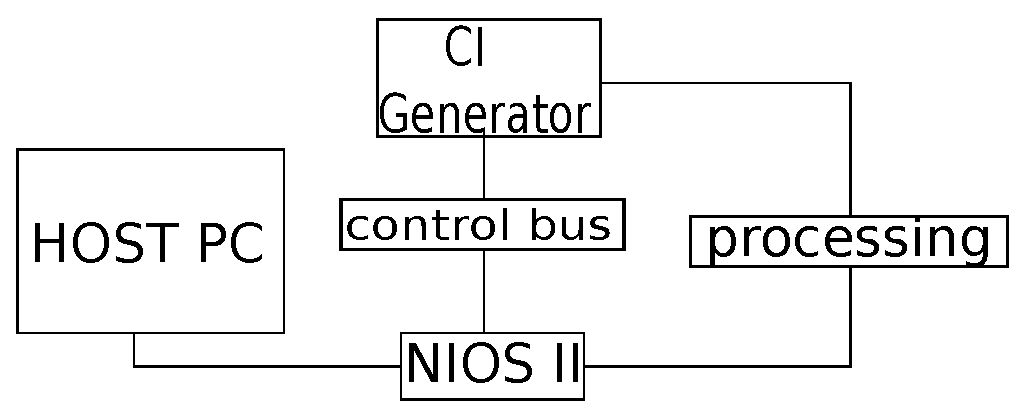
\includegraphics[width=6cm]{nios.eps}
\label{nios}} \hspace{0.5cm}
\subfigure[Schematic]{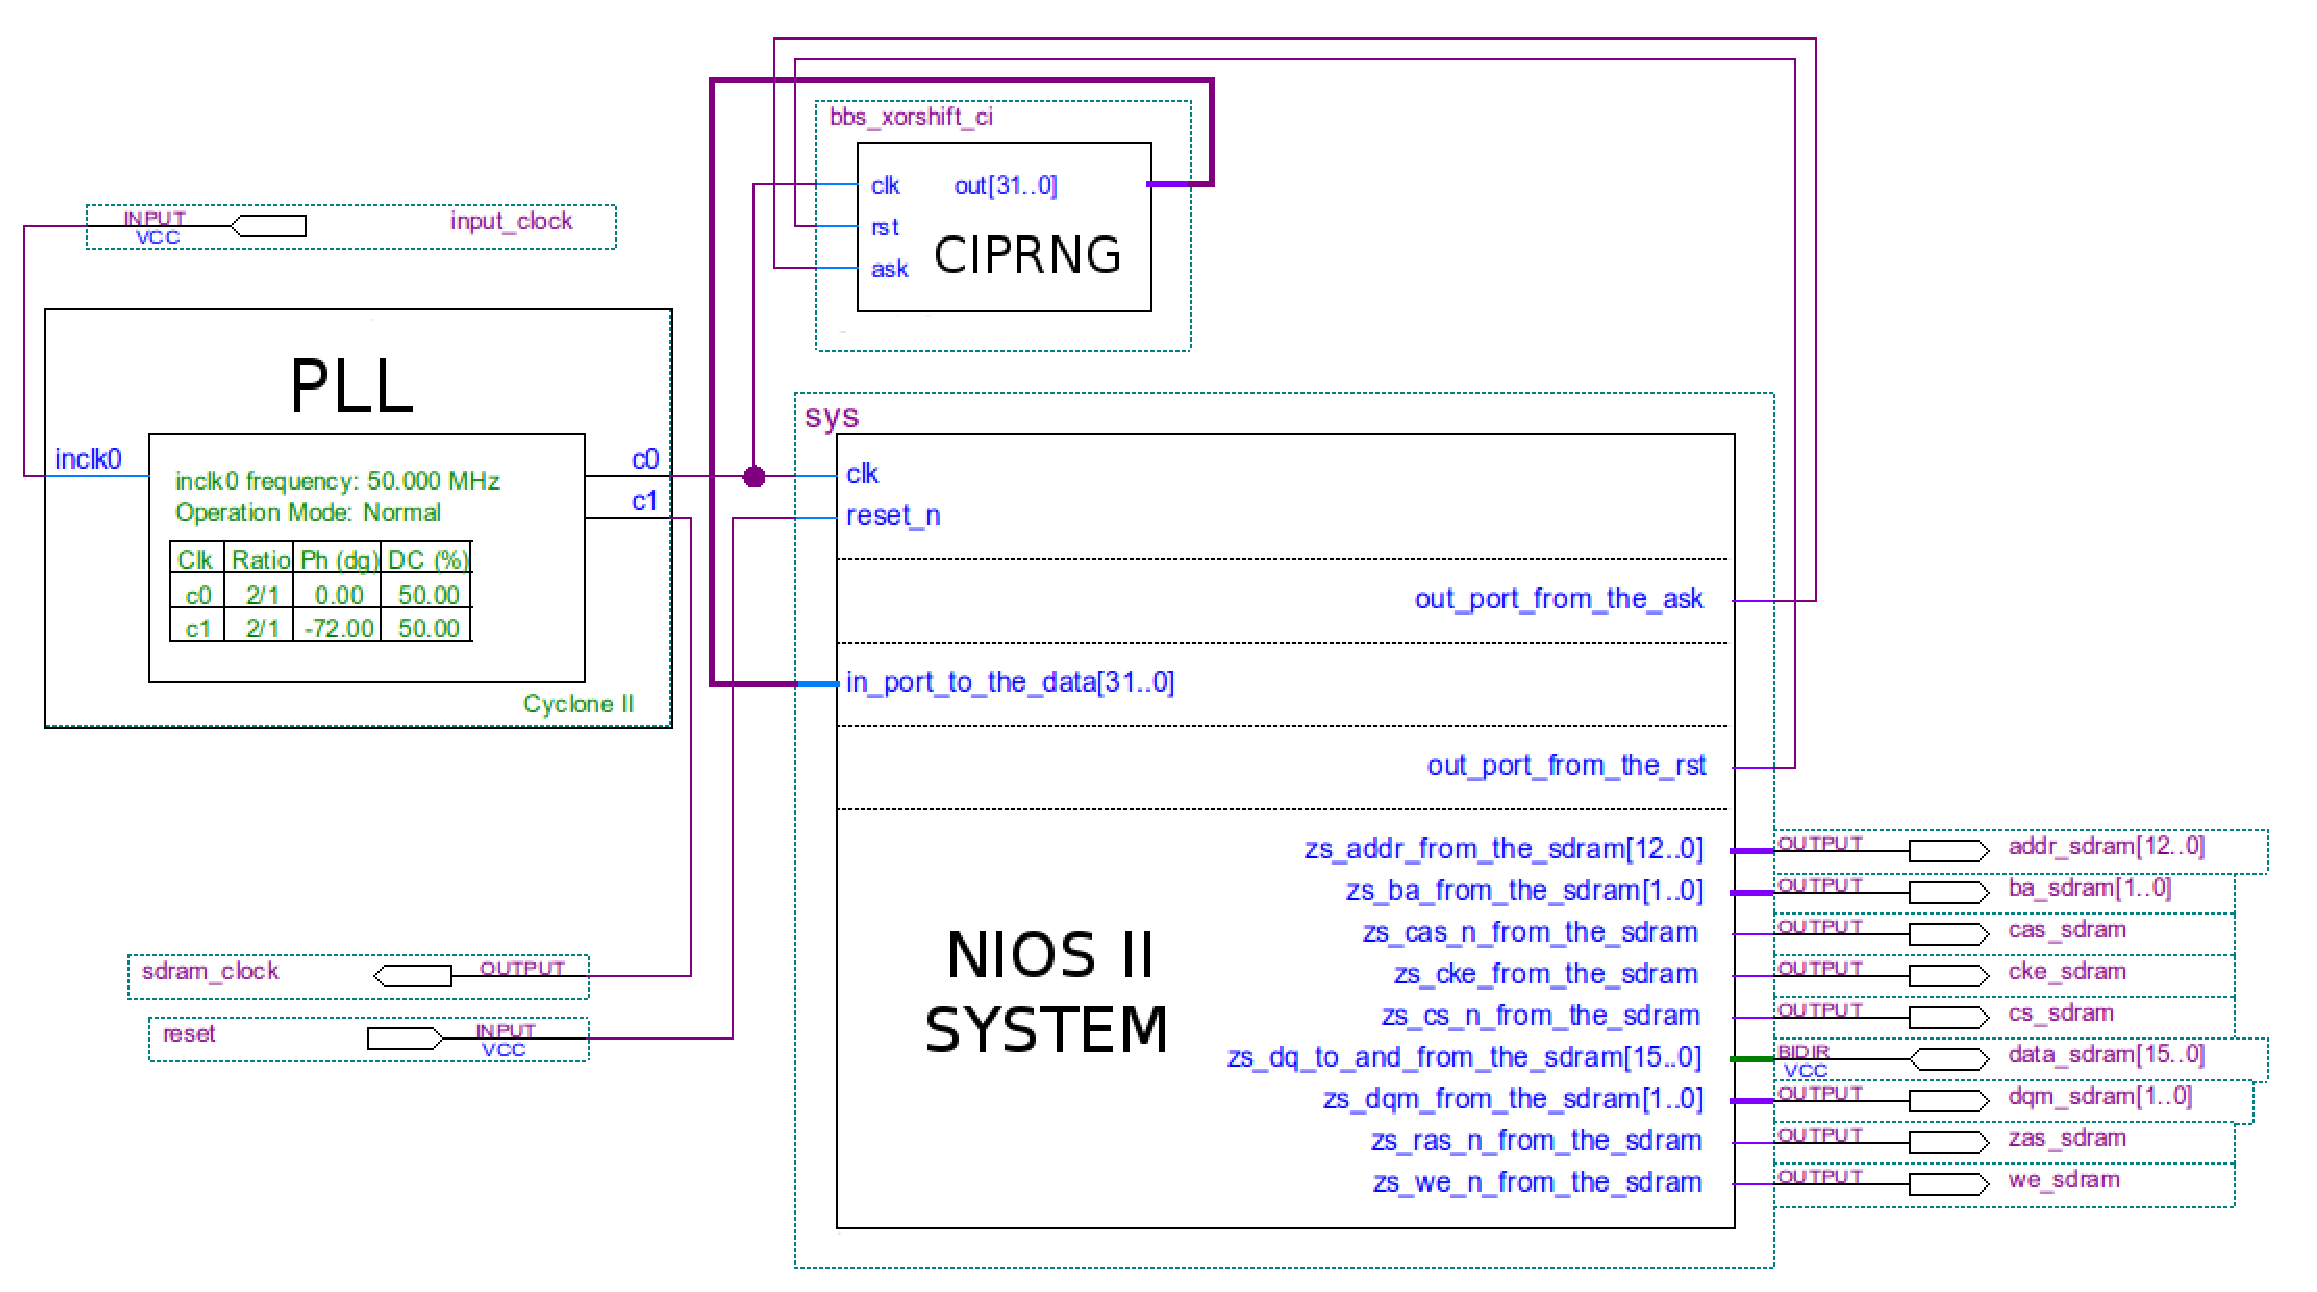
\includegraphics[width=\columnwidth]{nios2.eps}
\label{nios2}} \hspace{0.5cm}
\caption{NIOS II setting in FPGA}
\label{Spatial MSCs and LSCs of Lena}
\end{figure}

\section{Experimental protocol}
In this subsection, a concrete example is given: a watermark is encrypted and embedded into a cover image using the scheme presented in the previous section and  CIPRNG version 4 (BBS, XORshift). The carrier image is the well-known Lena, which is a 256 grayscale image, and the watermark is the $64\times 64$ pixels binary image depicted in Figure~\ref{Original images}.


\begin{figure}[!t]
\centering
\subfigure [The original image]{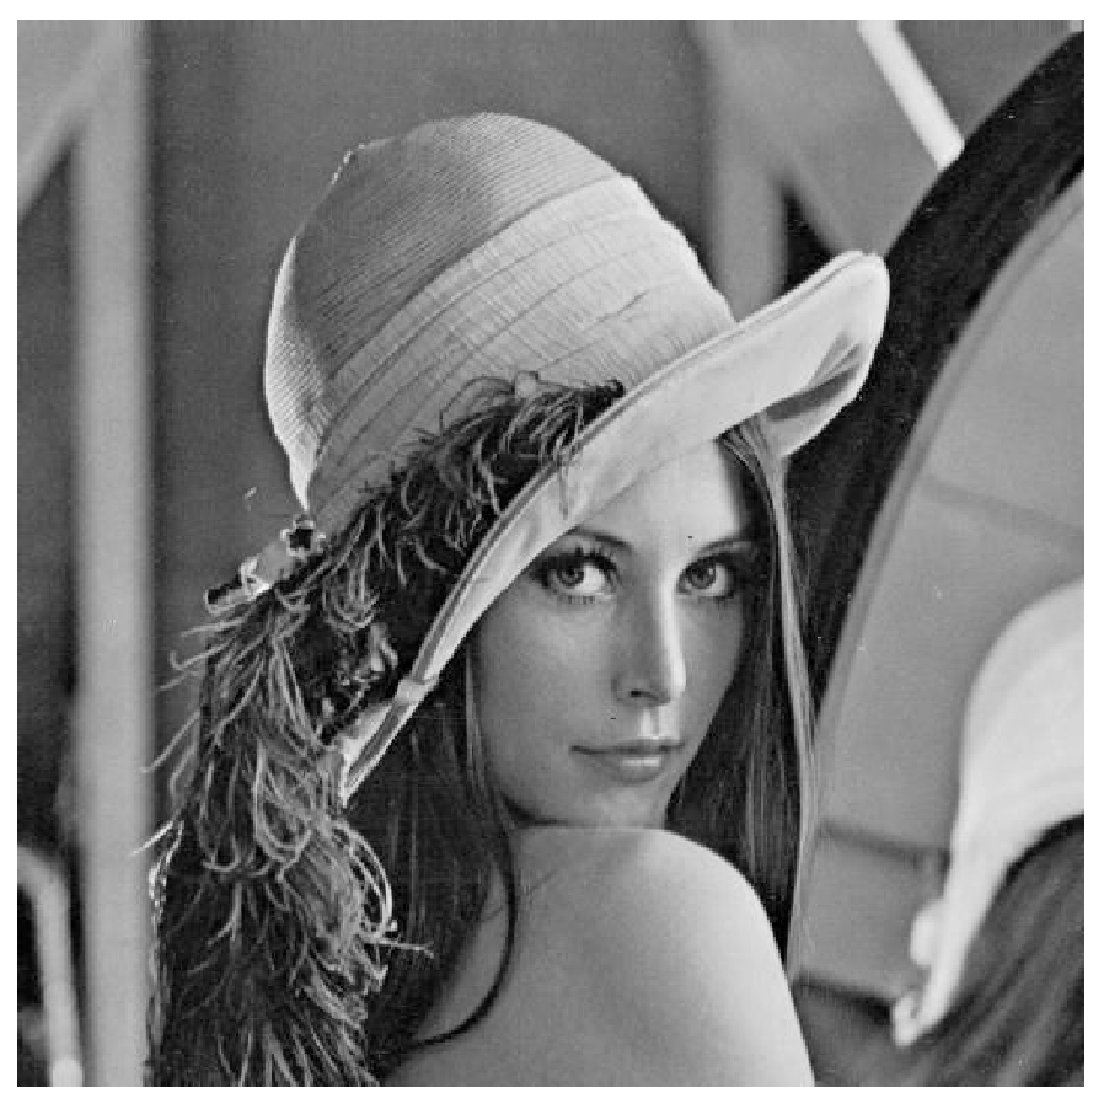
\includegraphics[scale=0.23]{lena512.eps}}
\hfil
\subfigure[The watermark]{
\includegraphics[scale=0.4]{invader1.eps}%
}
\caption{Original images}
\label{Original images}
\end{figure}


\begin{figure}[!t]
\centering
\subfigure [Differences with the original]{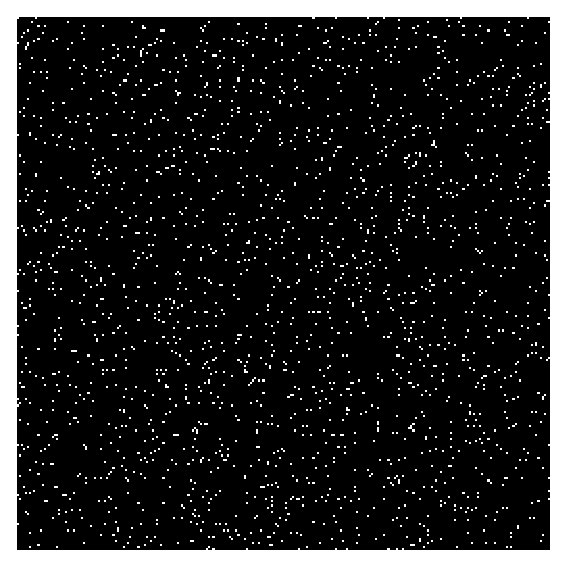
\includegraphics[scale=0.42]{lenaDiff2.eps}%
}
\hfil
\subfigure [Encrypted watermark]{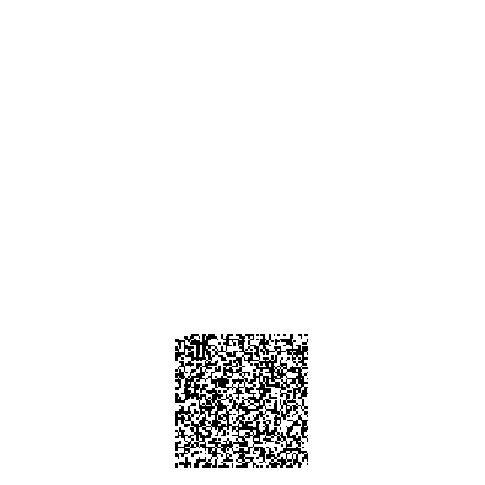
\includegraphics[scale=0.4]{invader_chiffre1.eps}%
}
\caption{Encrypted watermark and differences}
\label{Encrypted watermark and differences}
\end{figure}

The watermark is encrypted by using chaotic iterations: the initial state $x^{0}$ is the watermark, considered as a boolean vector, the iteration function is the vectorial logical negation, and the chaotic strategy $(S^{k})_{k\in \mathds{N}}$ is defined with CIPRNG version 4 (BBS, XORshift), where initial parameters constitute the secret key and $N=64$. Thus, the encrypted watermark is the last boolean vector generated by these chaotic iterations. An example of such an encryption is given in Figure~\ref{Encrypted watermark and differences}.


Let $L$ be the $256^3$ booleans vector constituted by the three last bits of each pixel of Lena and $U^k$ defined by the sequence:
\begin{equation}
\left\{
\begin{array}{lll}
U^{0} & = & S^{0} \\
U^{n+1} & = & S^{n+1}+2\times U^{n}+n ~ [mod ~ 256^3]%
\end{array}%
\right.
\end{equation}
The watermarked Lena $I_w$ is obtained from the original Lena, whose three last bits are replaced by the result of $64^2$ chaotic iterations with initial state $L$ and strategy $U$ (see Figure~\ref{Encrypted watermark and differences}).

The extraction of the watermark can be obtained in the same way. Remark that the map $\theta \mapsto 2\theta $ of the torus, which is the famous dyadic transformation (a well-known example of topological chaos~\cite{Dev89}), has been chosen to make $(U^{k})_{k \leqslant 64^2}$ highly sensitive to the strategy. As a consequence, $(U^{k})_{k \leqslant 64^2}$ is highly sensitive to the alteration of the image: any significant modification of the watermarked image will lead to a completely different extracted watermark, thus giving a way to authenticate media through the Internet.


Let us now evaluate the robustness of the proposed method.

\section{Implementations: from software to hardware}

We have been in charge to implement this chaotic iterations based watermarking
scheme on both software and hardware platforms, using one of the CIPRNGs we
previously studied. By doing so, we will be able to study the robustness
of the proposed hiding scheme, leading to the evaluation given in Section~\ref{robust}.

\subsection{Software Implementation: Experimental Protocol}

In this section, we details our software implementation of the information hiding application
 based on chaotic iterations presented in the previous sections: a watermark is encrypted and embedded into a cover image using the proposed scheme and some CIPRNGs. More precisely,
the CIPRNG(BBS, XORshift) version 4 has been chosen, since it is with good statistical performance and high efficiency.  The carrier image is the well-known Lena
already presented, which is here a $256 \times 256$ grayscale image, and the watermark is the $64\times 64$ pixels binary image depicted in Fig.\ref{Original images}.


\begin{figure}[!t]
\centering
\subfigure [The original image]{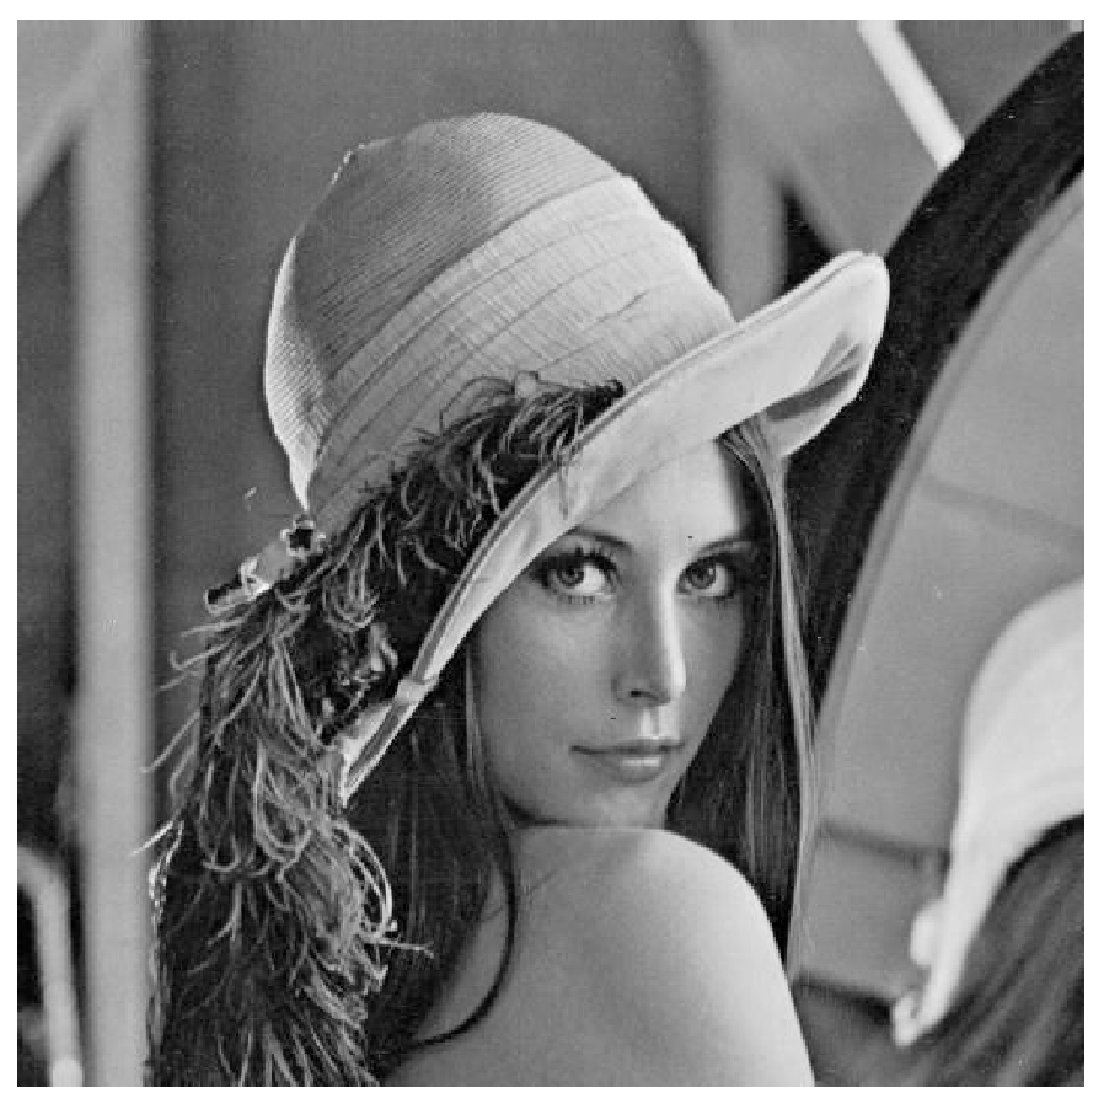
\includegraphics[scale=0.23]{lena512.eps}}
\hfil
\subfigure[The watermark]{
\includegraphics[scale=0.4]{invader1.eps}%
}
\caption{Original images}
\label{Original images}
\end{figure}


\begin{figure}
\centering
\subfigure[Output image]{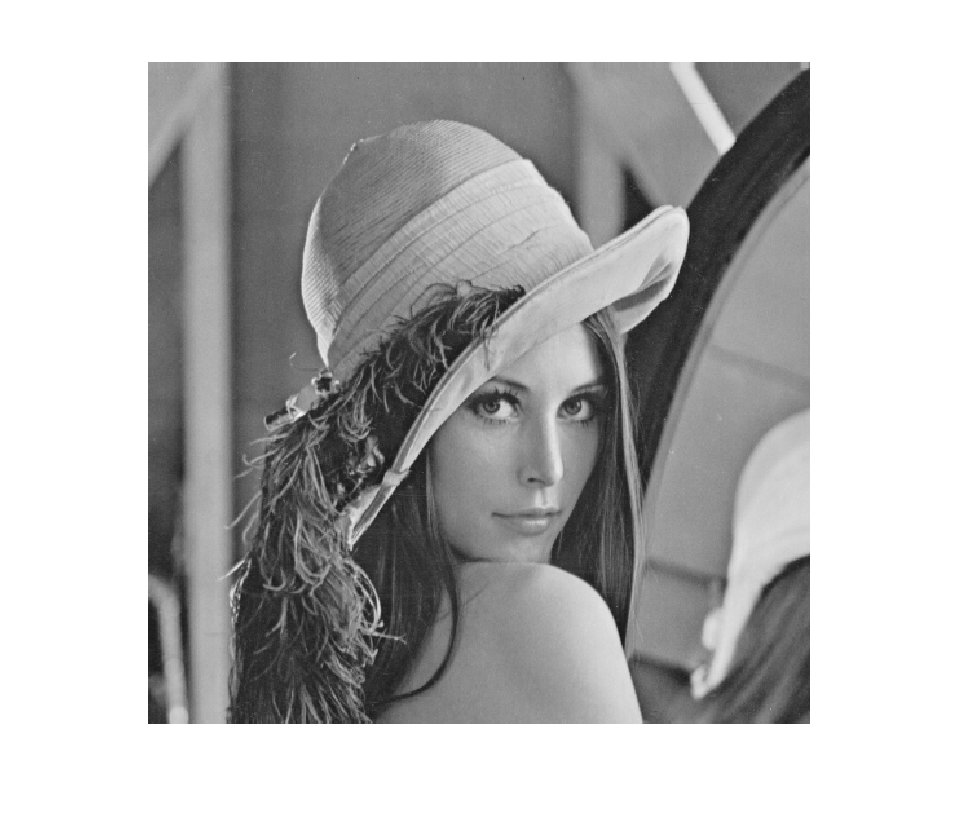
\includegraphics[scale=0.4]{output_lena.eps}}
\subfigure[Difference]{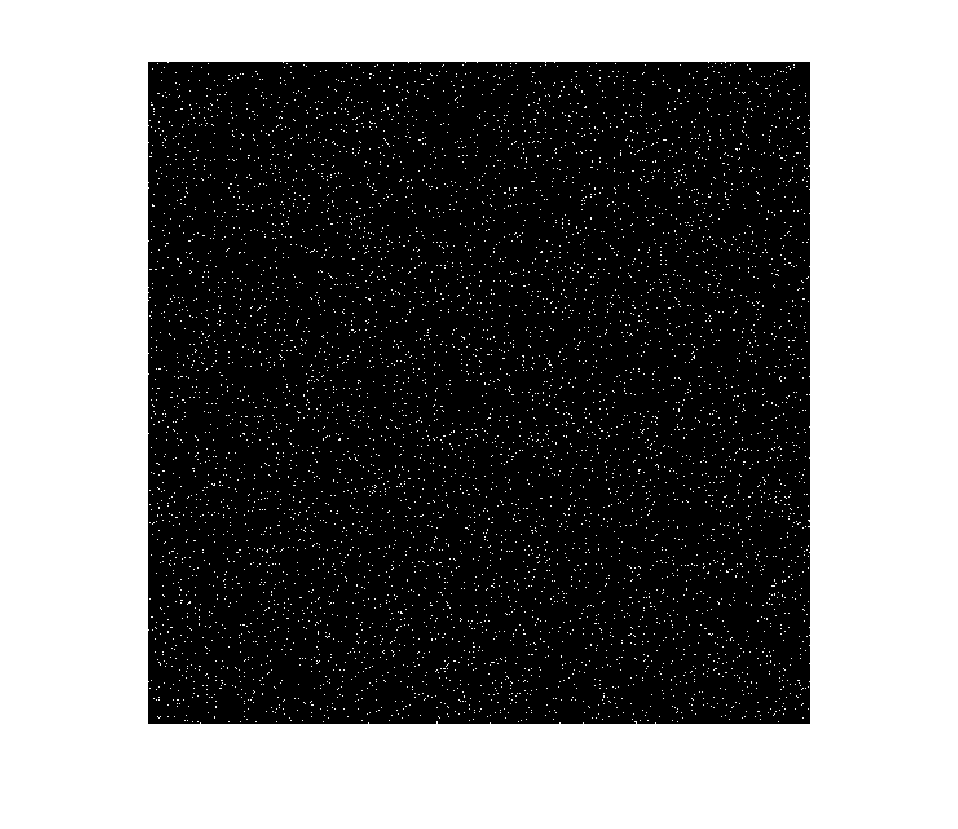
\includegraphics[scale=0.4]{diff.eps}}
\caption{The output of our watermarking application}
\label{java_end}
\end{figure}
The application has been computed using the JAVA language~\cite{java}. The watermark is encrypted by using chaotic iterations: the initial state $x^{0}$ is the watermark, considered as a Boolean vector, the iteration function is the vectorial logical negation, and the chaotic strategy $(S^{k})_{k\in \mathds{N}}$ is defined with CIPRNG(BBS, XORshift) version 4, whose initial parameters constitute the secret key and $N=64$.  
A simple windows interface has been implemented, as it is depicted in Fig.\ref{java application}-a.
The embedding file must firstly be chosen, as shown in Fig.\ref{java application}-b. 
Then the host image that will be used to carry the watermark must be selected (see Fig.\ref{java application}-c). Lastly, after processing, the output image is produced, and the differences between original image and encrypted image is produced (Fig.\ref{java_end}).

\begin{figure}
\centering
\subfigure [The start windows of our Java's watermarking application]{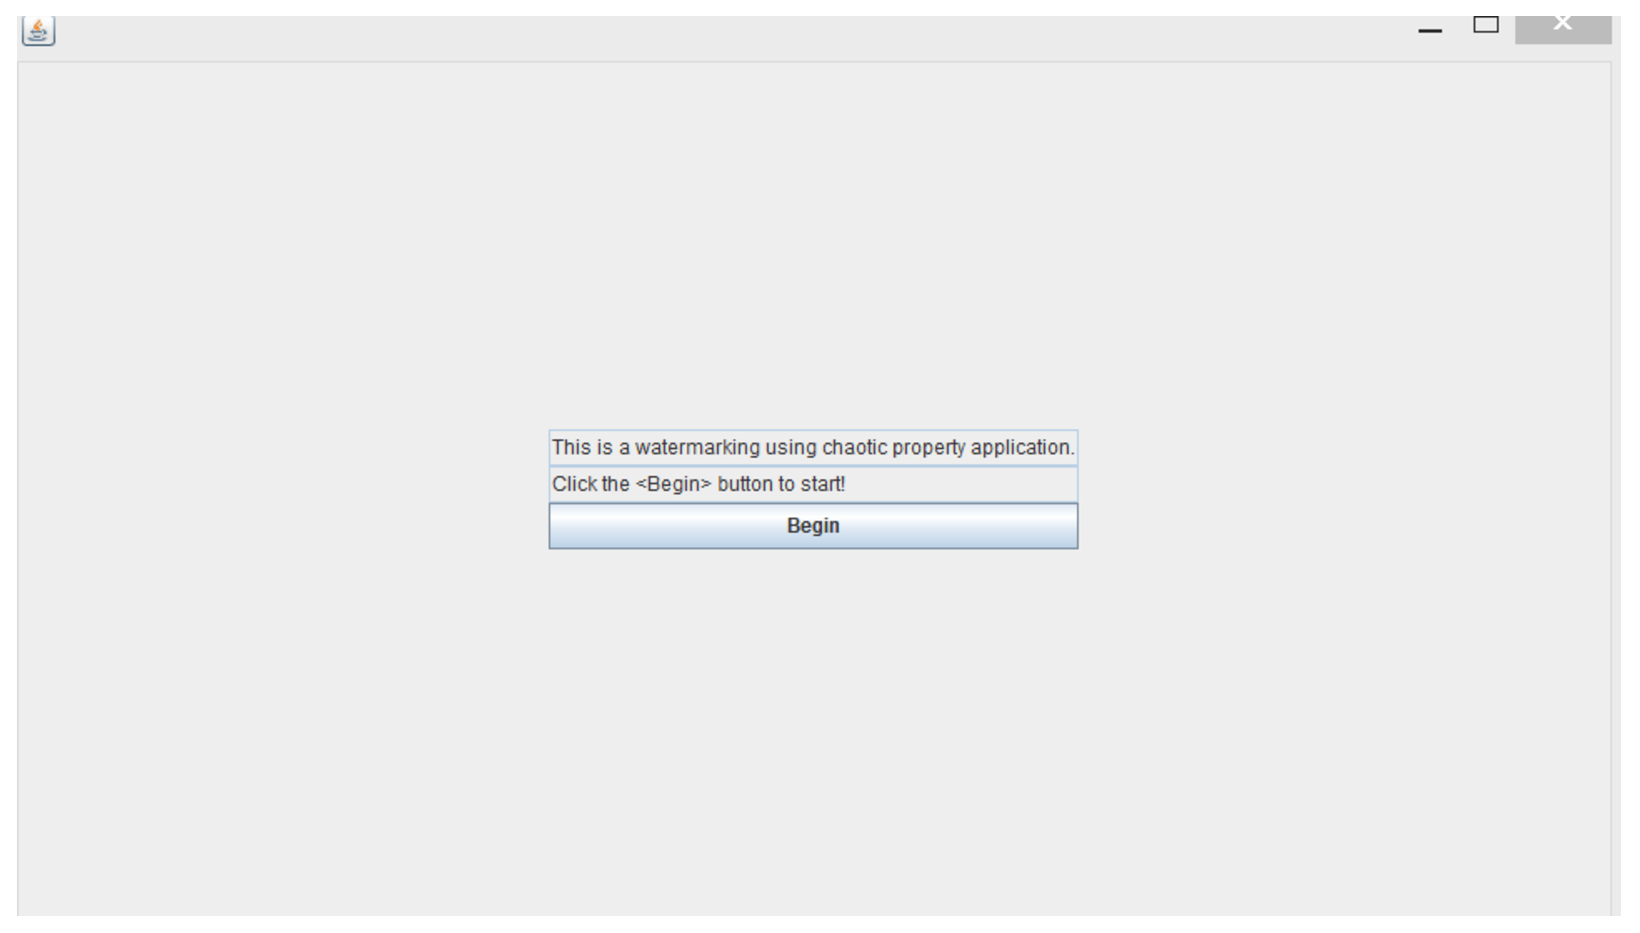
\includegraphics[scale=0.4]{start.eps}}
\subfigure [Choosing the contents to embed]{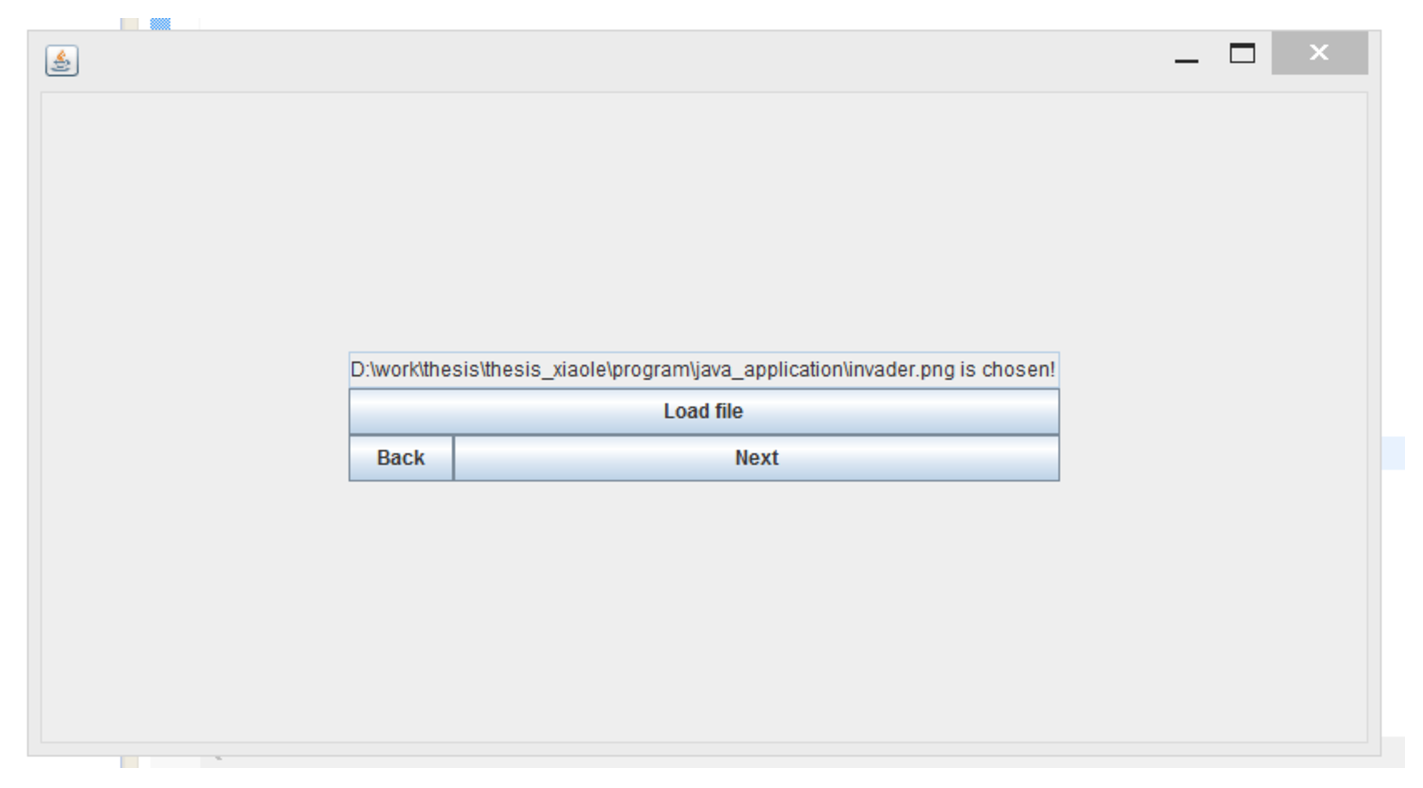
\includegraphics[scale=0.4]{chooseFile.eps}}
\subfigure [Choosing the contents to embed]{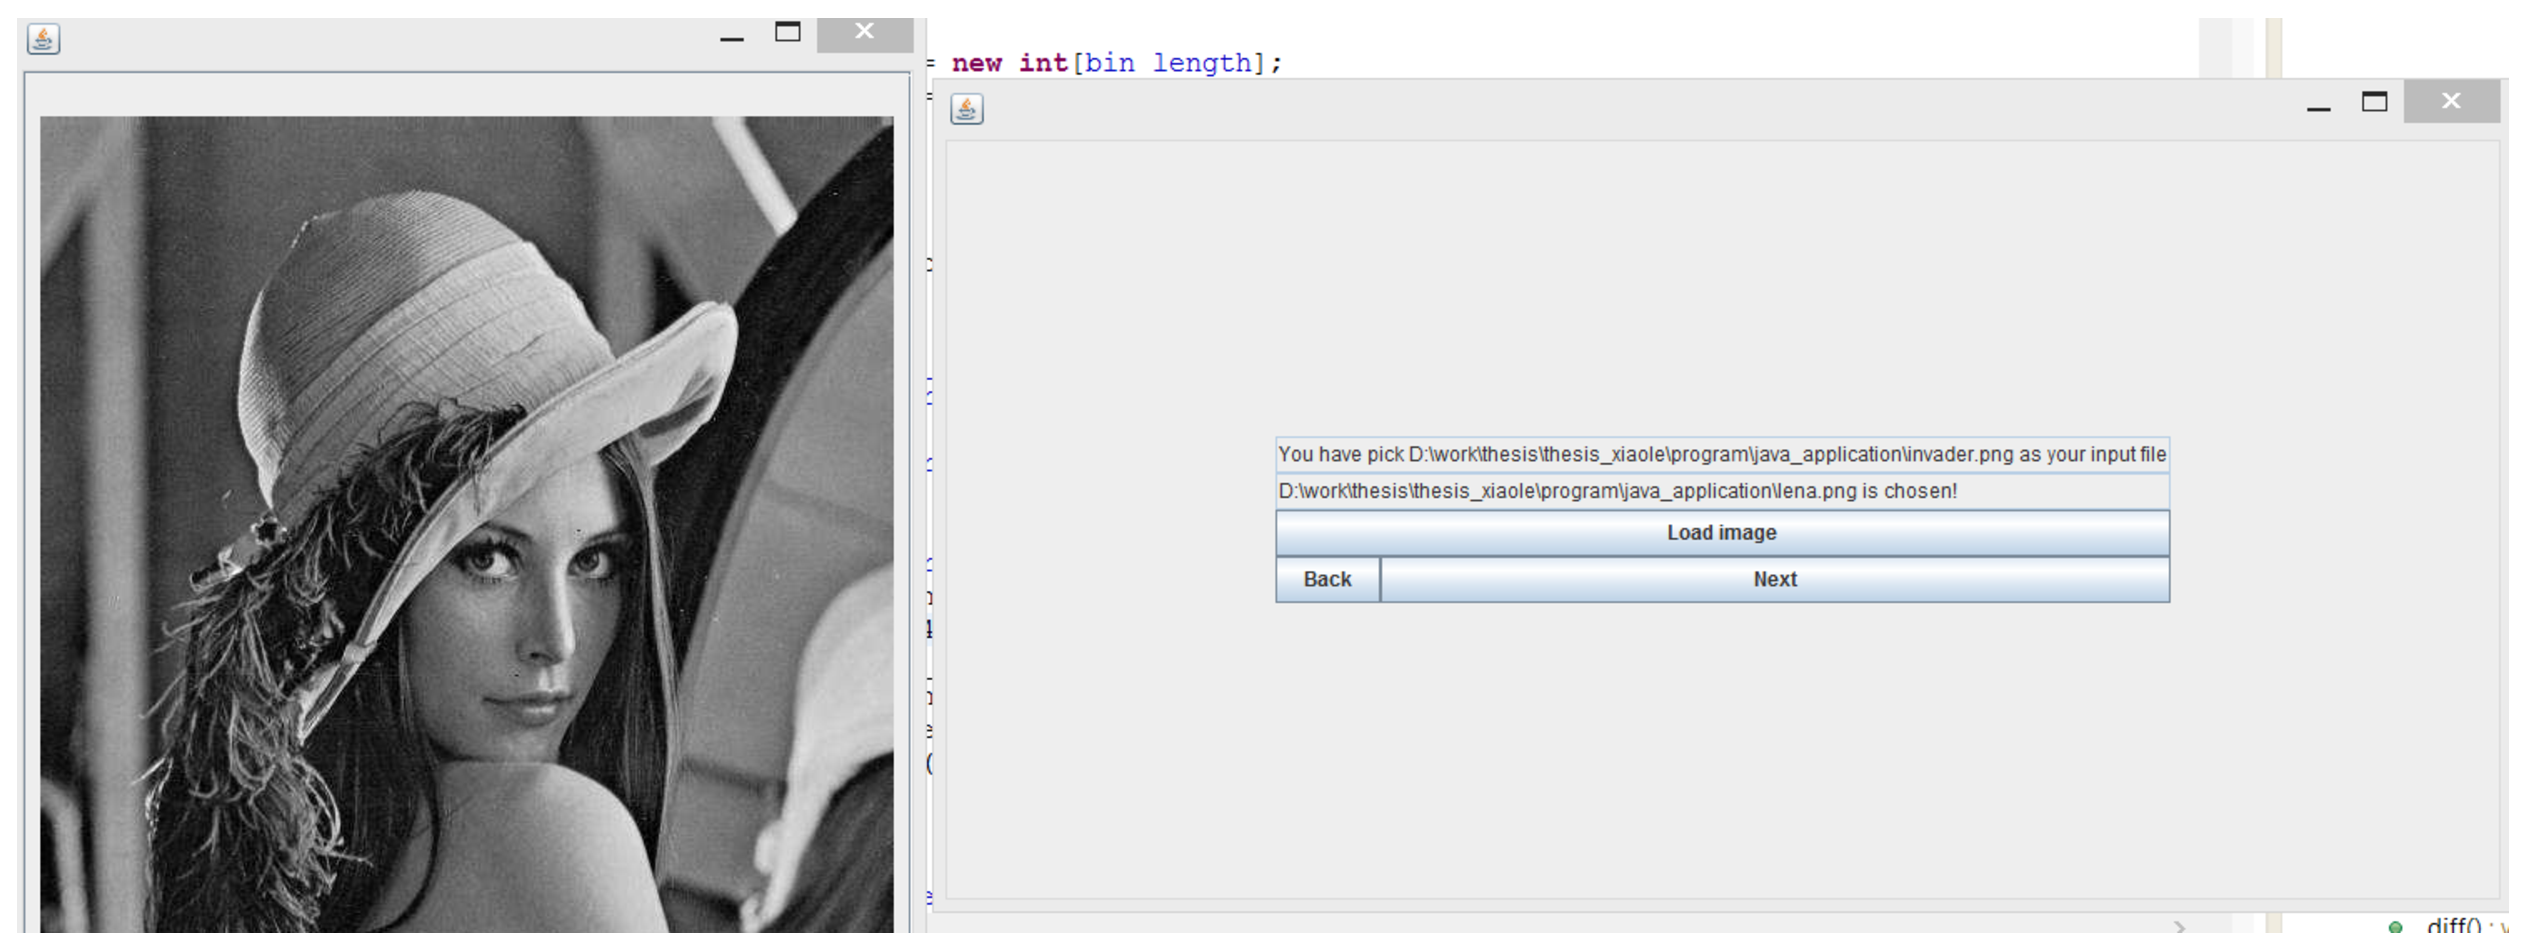
\includegraphics[scale=0.4]{chooseImage.eps}}
\caption{Java application for watermarking based on chaotic iterations}
\label{java application}
\end{figure}



\subsection{Hardware Implementation}

In this section, to show the effectiveness and lightweight of our approach using
chaotic iterations for both pseudorandom generations and information hiding,
we will shortly present our hardware implementation of the whole algorithm on a FPGA.
The 32-bit embedded-processor architecture designed specifically for the Altera family of FPGAs 
has been used for this application. Indeed, Nios II incorporates many enhancements over the original 
Nios architecture, making it more suitable for a wider range of embedded computing applications, 
from DSP to system-control, and to this watermarking scheme~\cite{nios}. 

Fig.\ref{nios} shows the structure of this application, 
the NIOS II system can read the image from the HOST computer side. 
Then the control bus allows
the CI generator to operate, in order to produce pseudorandom bits. 
Finally the processed results are transmitted back into 
the host. In Fig.\ref{nios2}, the NIOS II uses the most powerful 
version the CYCLONE II can support (that is, NIOS II/f). 
Then, $4$ KB on chip memory and $16$ MB SDRAM are set, and 
the $PLL$ device is used to enhance the clock frequency from $50$ 
to $200$ MHz. The data bus connects NIOS II system, and the generator is in 32 bits.


\section{Robustness evaluation}
\label{robust}
In what follows, the embedding domain is the spatial domain, CIPRNG(BBS,XORshift) version 4 
 has been used to encrypt the watermark, MSCs are the four first bits of each pixel (useful only in case of authentication), and LSCs are the three next bits.

To prove the efficiency and the robustness of the proposed algorithm, some
attacks are applied to our chaotic watermarked image. For each attack, a
similarity percentage with the watermark is computed, this percentage is the
number of equal bits between the original and the extracted watermark, shown
as a percentage. Let us notice that a result less than or equal to $50\%$
implies that the image has probably not been watermarked.

\subsubsection{Zeroing attack}

In this kind of attack, a watermarked image is zeroed, such as in Fig.\ref{fig:LenaAttack}(a). In this case, the results in Table. 1 have been obtained.
 For the sake of completeness, we 
recall the following results taken from Qianxue's thesis \cite{bibtexwangqianxue}.



\begin{figure}[htb]
\begin{minipage}[b]{.48\linewidth}
  \centering
 \centerline{\epsfig{figure=lennaDecoupe100px,width=3.3cm}}
  \centerline{(a) Cropping attack}
\end{minipage}
\hfill
\begin{minipage}[b]{0.48\linewidth}
  \centering
 \centerline{\epsfig{figure=lennaTourne25d.eps,width=3.3cm}}
  \centerline{(b) Rotation attack}
\end{minipage}
\caption{Watermarked Lena after attacks.}
\label{fig:LenaAttack}
\end{figure}




\begin{center}
\begin{footnotesize}
\begin{tabular}{|c|c||c|c|}
\hline
\multicolumn{2}{|c||}{UNAUTHENTICATION}  & \multicolumn{2}{c|}{AUTHENTICATION}\\ 
\hline
Size (pixels) & Similarity & Size (pixels) & Similarity \\
 \hline
10 & 99.31\% & 10 & 92.34\% \\
50 & 98.55\% & 50 & 57.11\% \\
100 & 92.40\% & 100 & 54.42\% \\
200 & 71.01\% & 200 & 50.93\% \\
\hline
\end{tabular}
\end{footnotesize}\\
\vspace{0.5cm}
\textbf{Table. 1}. ~Cropping attacks
\label{Table1}
\end{center}


In Fig.\ref{fig:Dechiffrement_invader}, the decrypted watermarks are shown after a crop of 50 pixels and after a crop of 10 pixels, in the authentication case.

\begin{figure}[htb]
\begin{minipage}[b]{1.0\linewidth}
  \centering
 \centerline{\epsfig{figure=invaderDechiffreDecoupe100px.eps,width=2cm}}
  \centerline{(a) Unauthentication ($50\times 50$).}
\end{minipage}
%
\begin{minipage}[b]{.48\linewidth}
  \centering
 \centerline{\epsfig{figure=invaderDechiffreDecoupeAuth100px.eps,width=2cm}}
  \centerline{(b) Authentication  ($50\times 50$).}
\end{minipage}
\hfill
\begin{minipage}[b]{0.48\linewidth}
  \centering
 \centerline{\epsfig{figure=invaderDechiffreDecoupeAuth50px.eps,width=2cm}}
  \centerline{(c) Authentication  ($10\times 10$).}
\end{minipage}
%
\caption{Extracted watermark after a cropping attack.}
\label{fig:Dechiffrement_invader}
%
\end{figure}


By analyzing the similarity percentage between the original and the
extracted watermark, we can conclude that in case of unauthentication, the
watermark still remains after a zeroing attack: the desired robustness is
reached. It can be noticed that zeroing sizes and percentages are rather
proportional.

In case of authentication, even a small change of the carrier image (a crop
by $10\times 10$ pixels) leads to a really different extracted watermark.
In this case, any attempt to alter the carrier image will be signaled, the
image is well authenticated.
\begin{center}
\begin{footnotesize}
\begin{tabular}{|c|c||c|c|}

\hline
\multicolumn{2}{|c||}{UNAUTHENTICATION}  & \multicolumn{2}{c|}{AUTHENTICATION}\\ 
\hline
Angle (degree) & Similarity & Angle (degree) & Similarity \\
 \hline
2 & 97.31\% & 2 & 74.45\% \\
5 & 94.02\% & 5 & 63.36\% \\
10 & 89.98\% & 10 & 52.77\% \\
25 & 80.84\% & 25 & 52.03\% \\
\hline
\end{tabular}
\end{footnotesize}\\
\vspace{0.5cm}
\textbf{Table. 2}. ~Rotation attacks
\end{center}

\subsubsection{Rotation attack}

Let $r_{\theta }$ be the rotation of angle $\theta $ around the center $%
(128, 128)$ of the carrier image. So, the transformation $r_{-\theta }\circ
r_{\theta }$ is applied to the watermarked image, which is altered as in Fig.\ref{fig:LenaAttack}. The results in Table. 2 have been obtained.




The same conclusion as above can be declaimed: this watermarking method
satisfies the desired properties.

\subsubsection{JPEG compression}

A JPEG compression is applied to the watermarked image, depending on a
compression level. Let us notice that this attack leads to a change of
the representation domain (from spatial to DCT domain). In this case, the results in Table 3 have been obtained.

\begin{center}
\begin{footnotesize}
\begin{tabular}{|c|c||c|c|}
\hline
\multicolumn{2}{|c||}{UNAUTHENTICATION}  & \multicolumn{2}{c|}{AUTHENTICATION}\\ 
\hline
Compression & Similarity & Compression & Similarity \\
 \hline
2 & 85.92\% & 2 & 58.42\% \\
5 & 70.45\% & 5 & 53.11\% \\
10 & 64.39\% & 10 & 51.02\% \\
20 & 53.94\% & 20 & 50.03\% \\
\hline
\end{tabular}
\end{footnotesize}\\
\vspace{0.5cm}
\textbf{Table. 3}. ~JPEG compression attacks
\end{center}

A very good authentication through JPEG attack is obtained. As for the
unauthentication case, the watermark still remains after a compression level
equal to 10. This is a good result if we take into account the fact that we
use spatial embedding.

\subsubsection{Gaussian noise}

Watermarked image can be also attacked by the addition of a Gaussian noise, depending on a standard deviation. In this case, the results in Table 4 have been obtained.


\begin{center}
\begin{footnotesize}
\begin{tabular}{|c|c||c|c|}
\hline
\multicolumn{2}{|c||}{UNAUTHENTICATION}  & \multicolumn{2}{c|}{AUTHENTICATION}\\ 
\hline
Standard dev. & Similarity & Standard dev. & Similarity \\
 \hline
1 & 81.00\% & 1 & 56.50\% \\
2 & 77.18\% & 2 & 51.92\% \\
3 & 67.01\% & 3 & 52.82\% \\
5 & 59.28\% & 5 & 51.76\% \\
\hline
\end{tabular}
\end{footnotesize}\\
\vspace{0.5cm}
\textbf{Table. 4}. ~Gaussian noise attacks
\end{center}


Once again we remark that good results are obtained, especially if we keep in
mind that a spatial representation domain has been chosen.


